\problemname{Treasure Spotting}
For Timmy's birthday his parents threw him a pirate themed party! A treasure is buried in the yard and now it is up to Timmy and his pirate crew to find it. Help the pirates find the treasure by letting them know who can see where the treasure is buried.

To make the game interesting, there are walls placed in the yard to
obscure vision. Each pirate has a field of view that determines what
they can see. Each pirate can see a certain distance away and can only
see in a semi-circle based on the direction they are looking (see
image below). A point cannot be seen in a pirate's field of view if
either another pirate or some part of a wall is directly between the
point that is being looked at and the pirate that is looking.  Each
pirate is a single point, and each wall is an infinitely thin line.

Which pirates can see where the treasure is buried?

\begin{figure}[h]
\begin{center}
 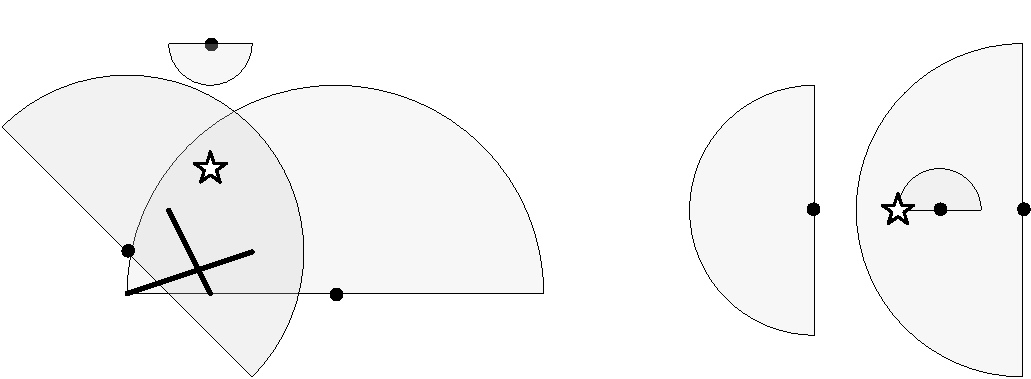
\includegraphics[width=0.7\textwidth]{sample.pdf}
 \caption{The left picture illustrates Sample Input 1 where the right-most pirate is the only one who can see the location of the buried treasure. The right picture illustrates Sample Input 2 where the middle pirate is the only one who can see the buried treasure.}
\end{center}
\end{figure}

\section*{Input}

The first line of input contains two integers $W$~($0 \leq W \leq 1 \, 000$), which is the number of walls and $P$~($1 \leq P \leq 1 \, 000$), which is the number of pirates.

The second line contains the coordinates of the treasure.

The next $W$ lines describe the walls. Each of these lines contains two coordinates $(x,y)$ and $(x',y')$ which are the two (distinct) endpoints of this wall.

The next $P$ lines describe the pirates. The $i$th of these lines contains two (distinct) coordinates $(x_i,y_i)$, which is the position of the $i$th pirate, and $(x_i',y_i')$, which is the furthest point that this pirate can see in the direction they are looking. That is, the radius of the semi-circle for this pirate is the distance between $(x_i, y_i)$ and $(x_i',y_i')$.

All coordinates are an $(x,y)$ integer pair with $|x|,|y| \leq 10^9$. No two pirates will have the same coordinate position, the treasure will not share a coordinate position with any pirate and no part of any wall will touch a pirate or the treasure. Note that walls can overlap in any way with other walls.

\section*{Output}

Display $P$ lines, one per pirate. The $i$th of these lines should display \texttt{visible} if the $i$th pirate can see where the treasure is buried and \texttt{not visible} otherwise.
